\title{This is title}
\author{
        This is author information\\
        Name\\
        Email
}
\date{}
\documentclass[12pt]{article}
\usepackage[margin=0.7in]{geometry}
\usepackage{graphicx}
\usepackage{float}
\usepackage{comment}
\usepackage{amsmath}
\usepackage{amssymb}
\usepackage{color}


\begin{document}
\maketitle

\begin{center}
\textbf{Abstract}
\end{center}
\noindent
This is Abstract section


\section{Introduction}
Introduction Section
\begin{enumerate}
\item Problem Statement
\end{enumerate}


\section{Background}
Background of Machine Learning and Deep Learning

{\color{blue} [Here summarize the Bengio paper \cite{bengio2009learning}]}

\begin{figure}[t!]
    \centering
    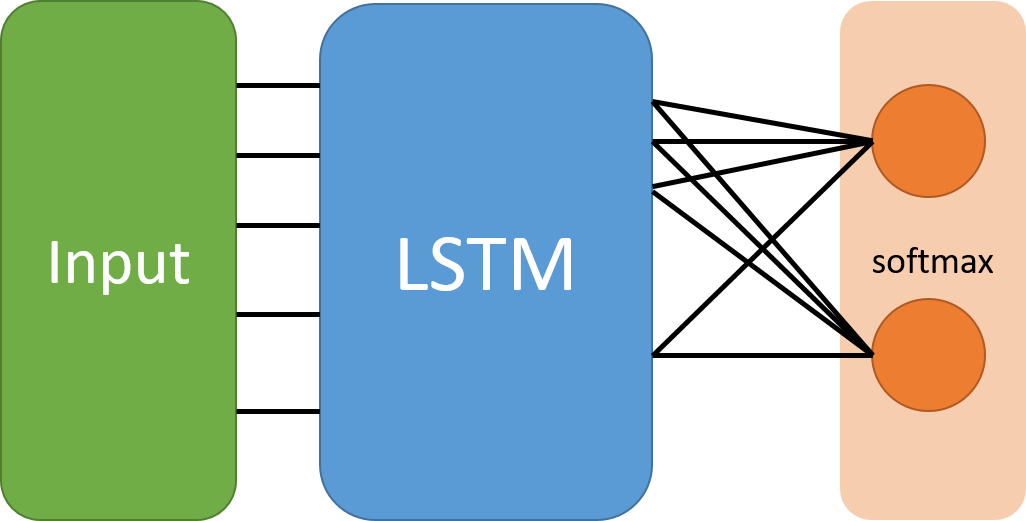
\includegraphics[width=0.5\textwidth]{pictures/FSFNN.png}
    \caption{blah blah blah.}
    \label{fig:lstm}
\end{figure}

{\color{blue} [LSTM should be in Figure \ref{fig:lstm}]}

\begin{enumerate}
\item Deep Learning
	\begin{enumerate}
	\item Summary of Recurrent Neural Network
		\begin{enumerate}
		\item Basic concept of recurrent neural network (RNN)\\
			RNN is a neural network but RNN has two input: one is from data, another is from previous output. Usually RNN is used with serial data. For example, human language sentence has series of words and data has time domain like driving data and stock data.
		\item Long Short Term Memory (LSTM) networks\\		
			Basic RNN has problem of long term dependency \cite{UnderstandingLSTMNetworks}. It means that RNN is not able to memorize long term knowledge. To solve the problem, LSTM is introduced by Hochreiter and Schmidhuber \cite{hochreiter1997long}. LSTM has cell state and the cell state can store long term memory. LSTM has four layer and three of them effect to cell state. Colah's blog \cite{UnderstandingLSTMNetworks} summarizes concept and purpose of each layers. The paper \cite{zaremba2014recurrent} describes LSTM in mathematical term. In this paper, I'm going to summarize the blog \cite{UnderstandingLSTMNetworks} and the paper \cite{zaremba2014recurrent}
			\begin{enumerate}
			\item Concept of each layers in LSTM\\
				Bengio mentioned on his paper \cite{bengio2009learning} that each layers in deep neural network have purpose. LSTM has four layers and four layers have different purpose. Colah's blog \cite{UnderstandingLSTMNetworks} summarizes it.\\
				The first layer is forget gate and effects to cell state and filters what data to forget or throw away. This layer is sigmoid layer with previous output and input data. The second layer is input gate and also effects to cell state and it decides what data to remember. The second layer is also sigmoid. The third layer is input modulation gate and also effects to cell state and it is tanh. Out put from second and third layers are added to previous cell state and updated for next cell state. Fourth layer is the last layer output gate and output is decided from result of output gate and updated cell state.
				
			\item Modeling LSTM in mathematical term\\
				LSTM is described in mathematical term in the paper \cite{zaremba2014recurrent}. I'm going to summarize it on this paper.\\
				Let\\
				$T_{n,m}: \mathbb{R}^n \rightarrow \mathbb{R}^m$ be an affine transform\\
				$x_t$ be current input \\
				$h_{t-1}$ be last output \\
				$h_{t}$ be current output \\
				$c_{t-1}$ be last cell state \\
				$c_{t}$ be current cell state \\

\[
\begin{bmatrix}
    input gate \\
    forget gate \\
    output gate \\
    input modulation gate
\end{bmatrix}
=
\begin{bmatrix}
    i \\
    f \\
    o \\
    g
\end{bmatrix}
=
\begin{bmatrix}
    sigm \\
    sigm \\
    sigm \\
    tanh
\end{bmatrix}
T_{2n,4n}
\begin{bmatrix}
    h_{t-1} \\
    x_{x}
\end{bmatrix}
\]
\[
=
\begin{bmatrix}
    sigm \\
    sigm \\
    sigm \\
    tanh
\end{bmatrix}
\begin{bmatrix}
    {T^{hi}}_{n,n} & {T^{xi}}_{n,n} \\
    {T^{hf}}_{n,n} & {T^{xf}}_{n,n} \\
    {T^{ho}}_{n,n} & {T^{xo}}_{n,n} \\
    {T^{hg}}_{n,n} & {T^{xg}}_{n,n}
\end{bmatrix}
\begin{bmatrix}
    h_{t-1} \\
    x_{x}
\end{bmatrix}
=
\begin{bmatrix}
    sigm \\
    sigm \\
    sigm \\
    tanh
\end{bmatrix}
\begin{bmatrix}
    {T^{hi}}_{n,n}h_{t-1} + {T^{xi}}_{n,n}x_{x} \\
    {T^{hf}}_{n,n}h_{t-1} + {T^{xf}}_{n,n}x_{x} \\
    {T^{ho}}_{n,n}h_{t-1} + {T^{xo}}_{n,n}x_{x} \\
    {T^{hg}}_{n,n}h_{t-1} + {T^{xg}}_{n,n}x_{x}
\end{bmatrix}
\]
Multiply two vector not matrix multiplication. Therefore,\\
\[
\begin{bmatrix}
    i \\
    f \\
    o \\
    g
\end{bmatrix}
=
\begin{bmatrix}
    sigm({T^{hi}}_{n,n}h_{t-1} + {T^{xi}}_{n,n}x_{x}) \\
    sigm({T^{hf}}_{n,n}h_{t-1} + {T^{xf}}_{n,n}x_{x}) \\
    sigm({T^{ho}}_{n,n}h_{t-1} + {T^{xo}}_{n,n}x_{x}) \\
    tanh({T^{hg}}_{n,n}h_{t-1} + {T^{xg}}_{n,n}x_{x})
\end{bmatrix}
\]

$\{i, f, o, g\}$ is a set of output from each layers.
The current cell state $c_t = f \cdot c_{t-1} + i \cdot g$
the current output $h_t = o \cdot tanh(c_t)$
			
				
			\end{enumerate}
		\end{enumerate}
	\end{enumerate}

\item Deep Learning Library\\
	\begin{enumerate}
	\item DL4J\\
	\item Theano\\
	\item Tensorflow\\
	\end{enumerate}

\item Machine Learning in Driving Data\\
\end{enumerate}


\section{Data Set}
Explain data\\


\section{Technical Approach}
Theory and Method\\
implementation with Tensorflow\\


\section{Experiment Result}
Result and Visualization\\


\section{Conclusion and Future work}
Conclusion and Future work\\


\section*{Reference}
Reference Section\\


\bibliographystyle{plain}
\bibliography{references.bib}


\end{document}


